\documentclass[fleqn,a4paper,12pt]{article}

%used Packages
\usepackage{standalone}		% Zum Einlesen aus anderen .tex-Files
\usepackage{geometry}		% Zur Bearbeitung des Layouts (Ränder,...)
\usepackage[german]{babel}
\usepackage[utf8]{inputenc}
\usepackage{amsmath}		% Mathematische Symbole
\usepackage{amssymb}     	% Nochmehr mathematische Symbole
\usepackage{dsfont}      	% Schriftsatz fuer Zahlenmengensymbole
%\usepackage{verbatim}   	% erweiterte Verbatim-Umgebung
\usepackage{alltt}       	% Quasi-Verbatim-Umgebung
\usepackage{fancyhdr}    	% Eigene Kopfzeilen
\usepackage{graphicx}    	% Zum Einbinden von Grafiken
							% Einbinden einer eps-Grafik geht so: includegraphics{path}
\usepackage{wrapfig}
\usepackage{lscape}
\usepackage{rotating}
\usepackage{epstopdf}

% Skalierung der Grafiken
\setlength{\unitlength}{1cm}

\frenchspacing               % Kein Extrafreiraum nach Satzzeichen
\setlength{\parindent}{0pt}  % Neue Absaetze nicht einruecken
%\sloppy                     % Schlampige Absatzformatierung
\fussy                       % Penible Absatzformatierung
\linespread{1.5}             % Zeilenabstand


% Seitenraender
\geometry{left=30mm, right=40mm, bottom=30mm}
				% Doc-class, Packageimports, fancy stuff
%%Seitenränder formatieren
\addtolength{\voffset}{-2cm}
\addtolength{\textheight}{0cm}
\addtolength{\hoffset}{0cm}
\addtolength{\textwidth}{2cm}
\addtolength{\headheight}{2cm} % fuer jeden Strichkode einen Zentimeter

% Font fuer Code 39
\font\xlix=wlc39 scaled 1200
\newcommand\barcode[1]{{\xlix@#1@}}

% Name, Matrikelnummer, Barcode
\newcommand\student[2]{
	\mbox{\scriptsize
		\begin{tabular}{@{}l@{}r@{}}
			\multicolumn{2}{@{}r@{}}{\barcode{#2}}\\
			#1&#2\\
		\end{tabular}}}

% Kopfzeile
\pagestyle{fancy}            % Eigene Kopfzeilen verwenden
\lhead{
	\small
	\textsc{Grundlagen der Signalverarbeitung \\
		WS 2017/2018 \\
		\"Ubung (\today)}
	\vfill}
\rhead{
	\begin{tabular}[b]{@{}rr@{}}
		\student{Philipp Badenhoop}{572693} &
		\student{Steven Lange}{568733} \\
		\student{Pascal Jochmann}{575056} &
		\student{Kevin Trogant}{572451}
\end{tabular}}			% Definition der Kopfzeile
%andere Definitionen
\providecommand{\R}{{\mathbb R}}
\providecommand{\N}{{\mathbb N}}
\providecommand{\Z}{{\mathbb Z}}
\providecommand{\Q}{{\mathbb Q}}
\providecommand{\C}{{\mathbb C}}
\providecommand{\F}{\mathcal{F}}
\providecommand{\less}{\setminus}
\providecommand{\inv}{{}^{-1}}
\providecommand{\Land}{\bigwedge}
\providecommand{\Lor}{\bigvee}			% Liste der zusätzlichen Commands und redefines

\begin{document}
    \section*{Übungsaufgabe 16}
    Gegebene Messwerte: \\
    \begin{center}
    \begin{tabular}{|c|c|c|}
        \hline 
        $n$ & $t_n$ & $f_n$ \\
        \hline
        0   &  0    & 3 \\
        1   &  1    & 3 \\
        2   &  3    & 9 \\
        3   &  4    & 15 \\
        \hline
    \end{tabular}
    \end{center}
    Wir wollen $f_{ap}(t) = c_1 t + c_0 t^0$ bestimmen. Aufstellen des Gleichungssystems liefert:
    \begin{align*}
        c_0 \sum_{n=0}^{3} t_n^0 t_n^0 + c_1 \sum_{n=0}^3 t_n^0 t_n^1 &= \sum_{n=0}^3 f_n t_n^0 \\
        \quad c_0 \sum_{n=0}^{3} t_n^1 t_n^0 + c_1 \sum_{n=0}^3 t_n^1 t_n^1 &= \sum_{n=0}^3 f_n t_n^1
    \end{align*}
    Einsetzen liefert:
    \begin{align*}
        4c_0 + 8c_1 &= 30 \\
        8c_0 + 26c_1 &= 90
    \end{align*}
    Einsetzen der Randbedingung $c_0 = 3$ liefert:
    \begin{align*}
        8c_1 &= 18  \Rightarrow c_1 = \frac{9}{4} \quad \textbf{Lsg 1} \\
        26c_1 &= 66 \Rightarrow c_1 = \frac{33}{13} \quad \textbf{Lsg 2}
    \end{align*}
    Für $c_0 = 3, c_1 = \frac{9}{4}$ ergibt sich:
    \begin{align*}
        E^2(c) = \sum_{n=0}^3 \left[ f_n - 3t_n^0 - \frac{9}{4}t_n^1 \right]^2 = \frac{117}{8} = 14.625
    \end{align*}
    Für $c_0 = 3, c_1 = \frac{33}{13}$ ergibt sich:
    \begin{align*}
        E^2(c) = \sum_{n=0}^3 \left[ f_n - 3t_n^0 - \frac{33}{13}t_n^1 \right]^2 = \frac{162}{13} \approx 12.462 
    \end{align*}
    \begin{figure}
        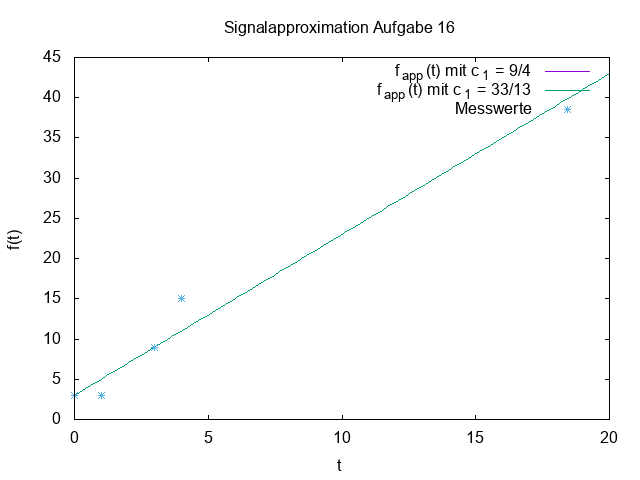
\includegraphics[width=\textwidth]{A16_plot.png}
        \caption{Grafische Darstellung}
    \end{figure}
\end{document}

